\documentclass{beamer}
\DeclareFontShape{OT1}{cmss}{b}{n}{<->ssub * cmss/bx/n}{} 
\usetheme{CambridgeUS}
\usepackage{amsmath}
\usepackage{amsfonts}
\usepackage{mathbbol}
\usepackage{xcolor} % before tikz or tkz-euclide if necessary
\usepackage{tkz-euclide} % no need to load TikZ
\usepackage{multirow}
\usepackage{lmodern}
\usepackage{bm}

\usepackage[
backend=biber,
style=authoryear-icomp,
sortlocale=de_DE,
natbib=true,
url=false, 
doi=true,
eprint=false
]{biblatex}
\addbibresource{../../Bibliography/main_ML.bib}



\titlegraphic{\includegraphics[width=2cm]{../../Figures/UAMS_RGB.png}
}


\title{Statistical Machine Learning\\ $p$-values and Multiple Testing}
\author{Horacio G\'omez-Acevedo\\ Department of Biomedical Informatics\\
	University of Arkansas for Medical Sciences}
\begin{document}
	\begin{frame}[plain]
		\maketitle
	\end{frame}
	
	\begin{frame}{Hypothesis test}
		\begin{itemize}
			\item A \textit{statistical hypothesis} $H$ ia a conjecture about the probability distribution of a population.
			\item A hypothesis $H$ is said to be \textit{simple} if the distribution of the population is completely specified by $H$. If not, then $H$ is called a \textit{composite} hypothesis.
			\item $H_0$ is called the \textit{null hypothesis} and $H_1$ the \textit{alternative hypothesis}.
			\item  We say that we commit a  \textit{type I error} if we decide to accept $H_1$, whereas in reality $H_0$ is true.
			\item  The probability of committing a type I error will be denoted by $\alpha$.
			\item Acceptance of $H_0$ whereas $H_1$ is true is called a \textit{type II error}. 
			\item  The probability of committing a type II error will be denoted by $\beta$.  
		\end{itemize}		

	\end{frame}

\begin{frame}{Error types}
	\centering
	\begin{tabular}{|c|c|c|}
		\hline
		&\multicolumn{2}{c|}{True State of Nature}\\
		\hline
		Decision & $H_0$ is TRUE & $H_1$ is TRUE\\
		\hline
		{\color{blue} Reject $H_0$}& TYPE I  & Correct  \\
		{\color{red} Accept $H_1$} & Error & Decision\\
		\hline
		{\color{blue} Accept $H_0$}& Correct  & TYPE II  \\
		{\color{red} Reject $H_1$} & Decision &  Error\\
		\hline
	\end{tabular}
\end{frame}

\begin{frame}{Example}
	A factory has packets of coffee with and adjusted weight of 500 grams. We assume that the weight of the packages is $N(500,50)$-distributed. Coffee packages are stored in containers (of unknown number). An error in a scale, some of the containers are filled up with packages of weight $N(490,50)$-distributed. To determine containers that have incorrectly weight the packages, we draw a sample of two packages from the given container. Based on the outcome of a 2-vector $(X_1,X_2)$ we will make a conjecture about the packages in that container. Namely
	\begin{equation*}
		\begin{split}
			H_0 & \text{: the population is } N(500,50)-\text{distributed}\\
			H_1 & \text{: the population is } N(490,50)-\text{distributed}
		\end{split}
	\end{equation*}
	Let's suppose our decision as\\
	\textit{If both $X_1$ and $X_2 \le 496$ then we accept $H_1$, otherwise we accept $H_0$. }
\end{frame}

\begin{frame}{Example (cont)}
	Let's define our \textit{critical region} $G$ as 
	\begin{equation*}
		G=\{(x_1,x_2)\in \mathbb{R}^2_+: x_1,x_2 \le 496\}
	\end{equation*}
	Then, we can formulate our decision as
	\begin{equation*}
		=
		\begin{cases}
			\text{if }(X_1,X_2) \in G & \text{then we choose $H_1$ as our conjecture}.\\
			\text{if }(X_1,X_2) \notin G & \text{then we choose $H_0$ as our conjecture}.\\
		\end{cases}	
		\end{equation*}
	\begin{figure}[h]
	\centering
	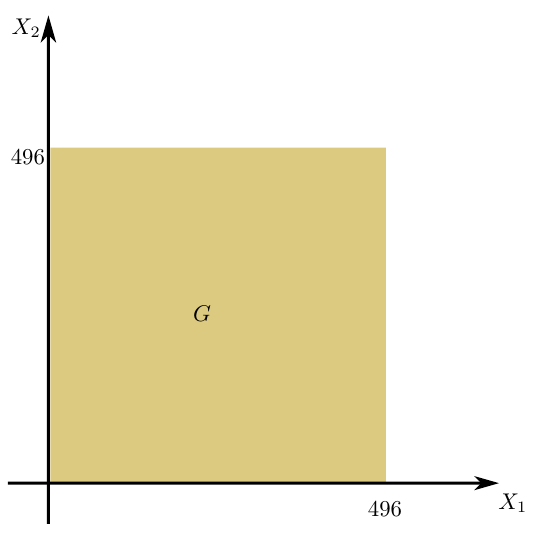
\includegraphics[scale=0.35]{../../Figures/fig_hypo_test_region.png}
\end{figure}		
	
	
\end{frame}

\begin{frame}{Calculating $\alpha$ and $\beta$}
	\begin{equation*}
		\begin{split}
			\alpha& = P(\text{acceptance of }H_1 | H_0\text{ is true}) \\ 
			& = P((X_1,X_2)\in G| \mu=500, \sigma^2=50) \\
			&=  P(X_1\le 496| \mu=500, \sigma^2=50) \cdot  P(X_2\le 496| \mu=500, \sigma^2=50)\\
			&= 0.081
		\end{split}
	\end{equation*}
	
	\begin{equation*}
		\begin{split}
			\beta& = P(\text{acceptance of }H_0 | H_1\text{ is true}) \\ 
			& = P((X_1,X_2)\notin G| \mu=490, \sigma^2=50) \\
			&= 1-P((X_1,X_2)\in G| \mu=490, \sigma^2=50) \\
			&=  1-P(X_1\le 496| \mu=490, \sigma^2=50) \cdot  P(X_2\le 496| \mu=490, \sigma^2=50)\\
			&= 0.356
		\end{split}
	\end{equation*}
\end{frame}

\begin{frame}{Hypothesis test}
	A \textit{Hypothesis test} is a collection
	\begin{equation*}
		(X_1,\ldots, X_n; H_0; H_1: G)
	\end{equation*}
 where $X_1,\ldots, X_n$ is a sample, $H_0$ and $H_1$ hypotheses concerning the probability distribution of the population and $G\subset \mathbb{R}^n$ a Borel set (meaning a collection of open sets)
 
 If $H_0$ is a simple statistical hypothesis. The \textit{level of significance} of the hypothesis test $(X_1,\ldots, X_n; H_0;H_1;G)$ is understood to be the number
 \begin{equation*}
 	\alpha = P_{X_1,\ldots, X_n}^{H_0}(G)
 \end{equation*}
Thus, we say that $\alpha$ represents the probability of committing a type I error.
\end{frame}

\begin{frame}{The power function}
	With our previous setup the $\beta$ could not be used for composite hypothesis. Thus, we have to define something more general. 
	\begin{itemize}
		\item Let $f(\cdot, \theta)_{\theta \in \Theta}$ be a family of probability densities 
		\item Let's assume that the population $X_1,\ldots, X_n$  has a probability density $f(\cdot,\theta)$ where $\theta \in \Theta$.  
		\item Let's assume that $H_0$ and $H_1$ are statements of the type
		\begin{equation*}
			H_0 \colon \theta \in \Theta_0 \quad \text{and} \quad H_1\colon \theta \in \Theta_1
		\end{equation*}
	where $\Theta_0 \cup \Theta_1= \Theta$ and $\Theta_1 \cap \Theta_1= \emptyset$.
	
	\end{itemize}
	For a fixed $\theta \in \Theta$, the probability distribution of the population is completely specified. Then, we define for every $\theta \in \Theta_1$
	\begin{equation*}
		\beta(\theta)= P_{X_1,\ldots, X_n}^\theta (G^c)
	\end{equation*}
	The expression $1-\beta(\theta)$ is called the \textit{power function} for $\theta \in \Theta_1$.
\end{frame}

\begin{frame}{Example (cont)}
	From our previous example, given is a $N(\mu, 50)$-distributed population, where $\mu \le 500$. 
	The family of probability densities $f(\cdot, \mu)$ where $\mu\le 500$ and 
	\begin{equation*}
		f(x,\mu)= \frac{1}{\sqrt{100 \pi}} \exp(\frac{-(x-\mu)^2}{100})
	\end{equation*}
	The parameter space is defined by $\Theta=(-\infty, 500]$. \\
	If we draw a sample $X_1$, $X_2$ of size 2 from this population. We can define $\Theta_0=\{500\}$ and $\Theta_1= (-\infty, 500)$. This corresponds to the following hypotheses
	\begin{equation*}
		H_0 \colon \mu = 500 \quad \text{against} \quad H_1 \colon \mu< 500
	\end{equation*}
If we choose the following critical region 
\begin{equation*}
	G= \{ (x_1,x_2)\in \mathbb{R}^2: x_1, x_2 \le 494.63 \}
\end{equation*}

	
\end{frame}

\begin{frame}{Example (cont)}
	Then, our 5-tuple $(X_1,X_2;H_0;H_1;G)$ constitutes a hypothesis test. 
	
	The size $\alpha$ of the critical region $G$ is $\alpha=0.05$, and the power function
	\begin{equation*}
		\begin{split}
			1-\beta(\mu)&= 1-P^\mu_{X_1,X_2}(G^c)= P^\mu_{X_1,X_2}(G)= P((X_1,X_2)\in G)\\
			&=P(X_1 \le 494.63 \text{ and } X_2 \le 494.63| \mu=\mu, \sigma^2=50) \\
			&=P(X_1 \le 494.63 | \mu=\mu, \sigma^2=50)\\
			&\quad  \cdot P(X_2\le 494.63 | \mu=\mu, \sigma^2=50) 
		\end{split}
	\end{equation*}
\end{frame}

\begin{frame}{Power function example}
	\begin{figure}[h]
	\centering
	\includegraphics[scale=0.8]{../../Figures/fig_power_function.png}
\end{figure}	
\end{frame}

\begin{frame}{Normally Distributed Case}
	Suppose we are dealing with a $N(\mu,\sigma^2)$-distributed population where both $\mu$ and $\sigma$ are unknown. If we wish to test the hypothesis
	\begin{equation*}
		H_0 \colon \mu=\mu_0 \text{ against } H_1 \colon \mu\ne \mu_0
	\end{equation*}
	Critical regions based on the likelihood ratio are of type
	\begin{equation*}
		G= \{(x_1,\ldots, x_n)\in \mathbb{R}^n : \left| \frac{\overline{x}-\mu_0}{s/\sqrt{n}} \right| \ge c\}
	\end{equation*}
	where $s^2= \frac{1}{n-1}\sum (x_i -\overline{x})^2$

	The outcome of the variable 
	\begin{equation*}
		T= \frac{\overline{X}-\mu_0}{S/\sqrt{n}}
	\end{equation*}
	is decisive in the choice to reject $H_0$ or not. This is called the \textit{Test statistic} for this hypothesis test. Under the $H_0$ the test statistics is $t$-distributed with $n-1$ degrees of freedom.
\end{frame}

\begin{frame}{Normally distributed case}
	The decision becomes
	\begin{equation*}
		\begin{split}
		\text{if }& |\frac{\overline{X}-\mu_0}{S/\sqrt{n}}| \ge c \text{, then assume }H_1\\
		\text{if }& |\frac{\overline{X}-\mu_0}{S/\sqrt{n}}| < c \text{, then assume }H_0
		\end{split}
	\end{equation*}
	And we have the following equivalence
	\begin{equation*}
		P(|\frac{\overline{X}-\mu_0}{S/\sqrt{n}}|\ge u)\le \alpha \iff u \ge c
	\end{equation*}
	If the outcome $u$ of $|\frac{\overline{X}-\mu_0}{S/\sqrt{n}}|$ satisfies 
	\begin{equation*}
		P(|\frac{\overline{X}-\mu_0}{S/\sqrt{n}}|\ge |u|)\le \alpha 
	\end{equation*}
	then, we accept $H_1$.
\end{frame}
\begin{frame}{$p$-values}
	The expression 
	\begin{equation*}
			P(|\frac{\overline{X}-\mu_0}{S/\sqrt{n}}|\ge |u|)
	\end{equation*}
	is called the $p$-value associated with the outcome $u$ of the test statistic.
	
	Therefore, we normally represent the decision rule
		\begin{equation*}
		\begin{split}
			\text{if }& P\text{-value} \le \alpha \text{, then assume }H_1\\
			\text{if }& P\text{-value} > \alpha \text{, then assume }H_0
		\end{split}
	\end{equation*}
\end{frame}

\begin{frame}{Cherry Picking Problem}
	Let's suppose we use the same data set and apply different test statistics at the $\alpha$ level of significance:
	\begin{itemize}
		\item $W_\alpha$ a Wilcoxon test,
		\item $P_\alpha$ a permutation test, and
		\item $T_\alpha$ a $t$-test.
	\end{itemize}
In this scenario, it may be possible that $W_\alpha$ may be true when $P_\alpha$ and $T_\alpha$ are not. 
\begin{equation*}
	P(W_\alpha \text{ or } T_\alpha \text{ or }P_\alpha| H) \ge P(W_\alpha|H) = \alpha
\end{equation*}
we will have an {\bf inflated} type I error by picking and choosing after the fact which test to report. 
\end{frame}


\begin{frame}{Cherry Picking Problem}
Similarly, 
if our intent was to conceal a side effect by reporting the results were not significant, we will inflate the Type II error and {\bf deflate} the power $\beta$ of our test by an after-the-fact choice as 

\begin{equation*}
	\beta=P(not(W_\alpha \text{and} P_\alpha \text{ and } T_\alpha)|K)\le(P(\text{ not } W_\alpha |K))
\end{equation*}

This quote from \citep{commonerrstat} is important to remember.

\begin{quote}
	We are not free to pick and choose among tests; any such conduct is unethical.
	{\bf Both the comparison and the test statistic must be specified in advance of examining the data.}
\end{quote}
\end{frame}


\begin{frame}{Multiple Testing}
	
	Consider the problem of simultaneously testing $m$ null hypotheses $H_j$, $j=1,\ldots, m$ and denote by $R$ the
	number of rejected hypothesis. In the frequentist setting, the situation can be summarized as 
	
	\begin{figure}[h]
		\centering
		\includegraphics[scale=0.8]{../../Figures/fig_fdr_table.png}
	\end{figure}
\end{frame}

\begin{frame}{Multiple Testing (cont)}	
	The $m$ hypotheses are assumed to be known in advance, while the number $m_0$ and $m_1$ of true and false null hypothesis are unknown parameter, $R$ is an observable random variable, and $S$, $T$, $U$, and $V$ are unobservable random variables. 
	
	In general, we want to minimize the number $V$ of false positives, or type I errors, and the number $T$ of false negative or type II errors. The standard approach is to pre-specify an acceptable type I error rate $\alpha$ that seek tests that minimize the type II error rate, within the class of tests with type I error rate $\alpha$. 
	

\end{frame}

\begin{frame}{Test for multiple comparisons}
	In terms of these random variables, we can define the main rates used in the present context.
When we are facing testing hypotheses of possibly thousands of significance tests, there are a 
number of alternatives dealing  	
\begin{itemize}
	\item The per-comparison error rate (PCER). The expected value of the number of type I error over the number of hypotheses
	\begin{equation*}
		PCER= \mathbb{E}(V)/m
	\end{equation*}
	\item The family-wise error rate (FWER). The probability of at least one type I error
	\begin{equation*}
		P(V\ge 1)
	\end{equation*}
	\item The false discovery rate (FDR) is the expected proportion of type I error among rejected hypotheses
	\begin{equation*}
		FDR=\mathbb{E}(V/R; R>0)=\mathbb{E}(V/R|R>0) P(R>0)
	\end{equation*}
\end{itemize}
\end{frame}


\begin{frame}{Ajusted $p$-values}
	To account for multiple hypothesis testing, one may calculate the adjusted $p$-values. Given a test procedure, the adjusted $p$-value correspoinding to the test of a single hypothesis $H_j$ can be defined as the level of the entire test procedure at which $H_j$ would just be rejected, given the values of all test statistics involved.
	
	Control of the FWER at level $\alpha$, the Bonferroni procedure rejects any hypothesis $H_j$ with $p$-value less than or equal to $\alpha/m$. 
\end{frame}

\begin{frame}{FDR control}
	The adjusted $p$-value goes according to this formula
	\begin{equation*}
		\tilde{p}_{r_i}= \min_{k=i,\ldots,m} \{ \min(mp_{r_k},1)\}
	\end{equation*}
	This adjustment leads to strong control of the FDR under the additional assumption of independence of the test statistics.
\end{frame}

\begin{frame}{References}
	Materials and some of the pictures are from \citep{pestman}, and \citep{speed}.
	\printbibliography 	
	
	I have used some of the graphs by hacking TiKz code from StakExchange, Inkscape for more aesthetic plots and other old tricks of \TeX
	
\end{frame}


\end{document}
